\documentclass[border=8pt]{standalone}
\usepackage[utf8]{inputenc}
\usepackage{tikz}
\usetikzlibrary{positioning}

\tikzset{
  entita/.style = {rectangle, draw, thick, fill=blue!8, minimum width=28mm, minimum height=14mm, font=\small},
  attr/.style   = {circle, draw, thick, fill=white, minimum size=5pt, inner sep=0},
  pk/.style     = {circle, draw, thick, fill=black, minimum size=5pt, inner sep=0},
  link/.style   = {thick},
  et/.style     = {font=\footnotesize}
}

\begin{document}
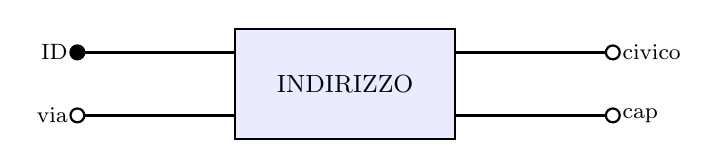
\begin{tikzpicture}

  \node[entita] (E) {INDIRIZZO};

  \node[pk]   (id)  at (-3.4, 0.4){}; \draw[link] (-1.4, 0.4)--(id);  \node[et,left] at (id)  {ID};
  \node[attr] (via) at (-3.4,-0.4){}; \draw[link] (-1.4,-0.4)--(via); \node[et,left] at (via) {via};
  \node[attr] (civ) at ( 3.4, 0.4){}; \draw[link] ( 1.4, 0.4)--(civ); \node[et,right] at (civ) {civico};
  \node[attr] (cap) at ( 3.4,-0.4){}; \draw[link] ( 1.4,-0.4)--(cap); \node[et,right] at (cap) {cap};

\end{tikzpicture}
\end{document}
